\documentclass[a4paper, 12pt]{article}


\usepackage[french]{babel}
\usepackage[utf8]{inputenc}
\usepackage[T1]{fontenc}
\usepackage{lmodern}
\usepackage{listings}
\usepackage{graphicx}
\usepackage{amsmath}
\usepackage{amsfonts}
\usepackage{amssymb}
\usepackage{caption}
\usepackage{subcaption}
\usepackage[usenames,dvipsnames]{xcolor}


\setcounter{secnumdepth}{4}
% TAILLE DES PAGES (A4 serré)

\setlength{\parindent}{0pt}
\setlength{\parskip}{1ex}
\setlength{\textwidth}{17cm}
\setlength{\textheight}{24cm}
\setlength{\oddsidemargin}{-.7cm}
\setlength{\evensidemargin}{-.7cm}
\setlength{\topmargin}{-.5in}

% Commandes de mise en page
\newcommand{\fichier}[1]{\emph{#1}}
\newcommand{\nom}[1]{\emph{#1}}
\newcommand{\Fig}[1]{Fig \ref{#1} p. \pageref{#1}}
\newcommand{\itemi}{\item[$\bullet$]}

% Commandes de maths
\newcommand{\fonction}[3]{#1 : #2 \to #3}
\newcommand{\intr}[2]{\left[ #1 ; #2 \right]}
\newcommand{\intn}[2]{\left[\![ #1 ; #2 \right]\!]}
\newcommand{\intro}[2]{\left] #1 ; #2 \right[}
\newcommand{\intrsod}[2]{\left[ #1 ; #2 \right[}
\newcommand{\ps}[2]{\langle #1, #2 \rangle}
\newcommand{\mdelta}[1]{\boldsymbol{\delta_{#1}}}
%% \newcommand{\mdelta}[1]{\delta_{\textbf{#1}}}

\pagenumbering{arabic}
\graphicspath{{images/}}

\title{ASM-TP1 : Cancer de la prostate} 
\author{Pierre Petitbon \and Florian Privé \and Xinrui Xu}
\date{}

\begin{document}

\maketitle

\section{Analyse préliminaires des données}

\begin{enumerate}

\item On visualise sous R la matrice de corrélation entre lpsa et les 8 prédicteurs. 

\begin{center}
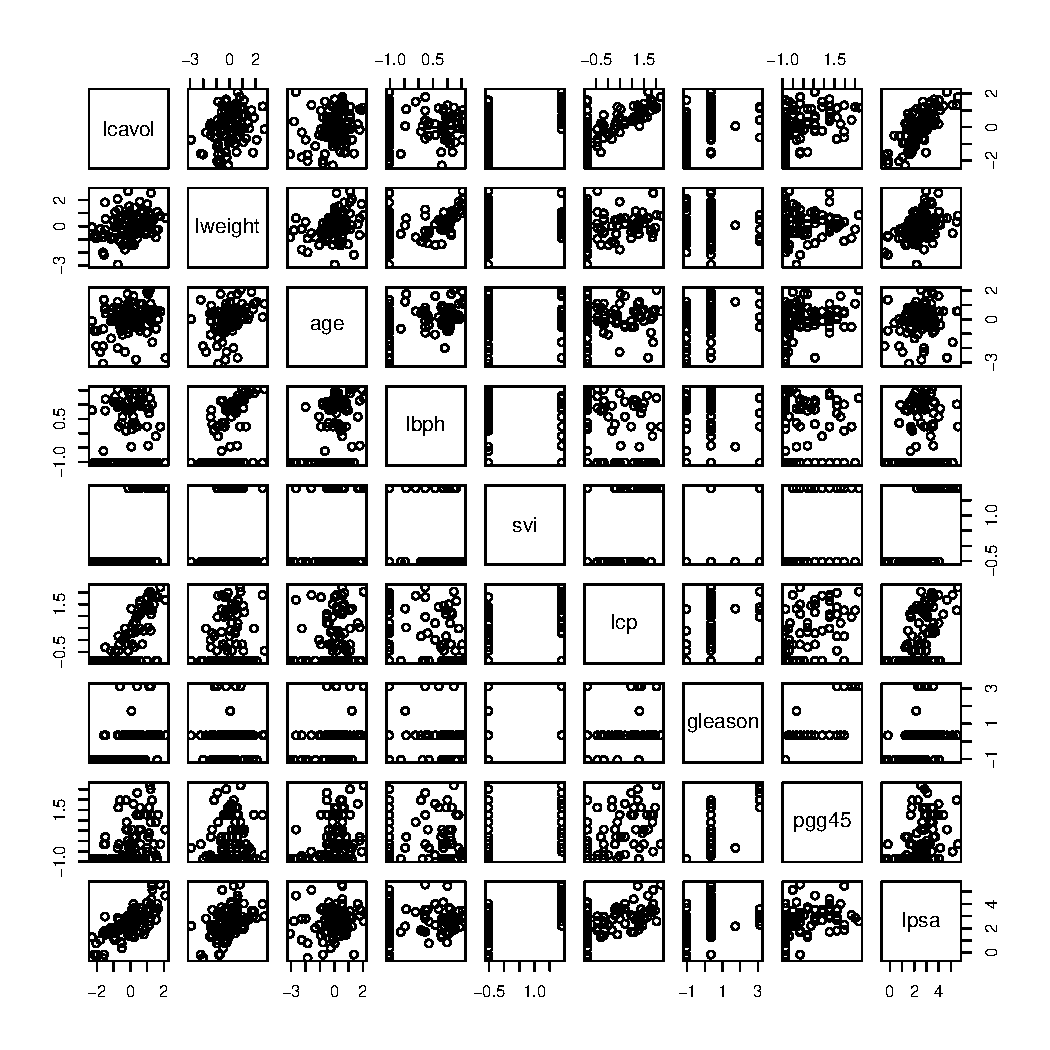
\includegraphics[scale=0.5]{Rplots.pdf}
\captionof{figure}{Rplots}
\label{fig1}
\end{center}

À partir du graphe précédent, on peut voir que certains facteurs sont corrélés ou pas avec lpsa. Pour cela, il suffit de regarder si le nuages de points forme plus ou moins une ellipse. 

\begin{tabular}{|p{0.5cm}|p{1.5cm}|p{1.5cm}|p{1.5cm}|p{1.5cm}|p{1.5cm}|p{1.5cm}|p{1.5cm}|p{1.5cm}|}
  \hline
       & lcavol & lweight & age & lbph & svi & lcp & gleason & pgg45 \\
  \hline
  lpsa & corrélé & non 

   corrélé & non 

    corrélé & non

     corrélé & corrélé & corrélé & non

      corrélé & non

       corrélé \\
  \hline 
\end{tabular}


\item 
À partir du graphe précédent, on peut aussi conjecturer s'il y a corrélation entre les prédicteurs.

\begin{tabular}{|p{1.4cm}|p{1.4cm}|p{1.4cm}|p{1.4cm}|p{1.4cm}|p{1.4cm}|p{1.4cm}|p{1.4cm}|p{1.4cm}|p{1.4cm}|}
  \hline
       & lcavol & lweight & age & lbph & svi & lcp & gleason & pgg45 \\
  \hline
  lcavol &  & non 

  corrélé & non 

   corrélé & corrélé & corrélé & corrélé & corrélé & corrélé \\
  \hline 
  lweight & non 

  corrélé & & non

  corrélé & non

  corrélé & non 

  corrélé & corrélé & corrélé & non

   corrélé \\
   \hline
   age & non 

   corrélé & non 

   corrélé &  & corrélé & corrélé & non 

   corrélé & corrélé & non 

   corrélé \\
   \hline
   lbph & corrélé & non 

   corrélé & corrélé & & corrélé & 
   non 

   corrélé & non 

   corrélé &
   non

   corrélé \\
   \hline
   svi & corrélé & non 

   corrélé & corrélé & corrélé & & corrélé & non 

   corrélé & corrélé \\
   \hline
   lcp & corrélé & corrélé & non 

   corrélé & non 

   corrélé & corrélé &  & corrélé & non

    corrélé \\
    \hline
    gleason & corrélé & corrélé & corrélé & non 

    corrélé & non 

    corrélé & corrélé & & corrélé \\
    \hline
    pgg45 & corrélé & non 

    corrélé & non 

    corrélé & non 

    corrélé & corrélé & non 

    corrélé & corrélé & \\
    \hline

\end{tabular}

\end{enumerate}



\section{Régression linéaire. Méthodes des moindres carrés.}

\begin{enumerate}
\item
La régression classique consiste à estimer les coefficients $\beta_{j}$ intervenant dans la relation suivante :

$ Y_{i} = \sum\limits_{j=1}^6 \beta_{j} x_{ij} + \beta_{0} + \sum\limits_{l=2}^4 \beta_{gleason, l} \mathbf{1}_{x_{gleason, i}=l} + \epsilon_{i} $

où $Y$ représente lpsa et les $x_{j}$ représentent les prédicteurs.  

D'après les résultats obtenus, les prédicteurs qui semblent influer le plus sur lpsa sont :
\begin{itemize}
\item lcavol (***) : on prend un risque très faible (p-valeur $=2.9x10^{-8}\%$) en disant que $\beta_{lcavol} \neq 0$.
\item lweight (**) : p-valeur $=0.25\%$.
\item svi (**) : p-valeur $=0.31\%$.
\end{itemize}
On prend également peu de risque en disant que $\beta_{lweight} \neq 0$ et $\beta_{svi} \neq 0$ 
\begin{itemize}
\item age (*) : p-valeur $=4.4\%$.
\end{itemize}

\item La p-valeur correspondant à la variable lcp est très élevée ($19\%$), donc l'estimation de $\beta_{lcp}$ est peu précise. C'est pourquoi il est préférable de calculer un intervale de confiance pour $\beta_{lcp}$.

L'intervalle de confiance au seuil de $1\%$ trouvé est $[-0.52, 0.17]$. Cet intervalle recouvre à la fois des valeurs négatives et positives, donc ce qui confirme le manque de précision dans l'estimation du $\beta_{lcp}$ puisqu'on est même pas sûre de son signe.

Si on décide d'ignorer lcavol et svi, on trouve un nouvel intervalle de confiance qui est : $[0.10, 0.75]$. On remarque que la largeur de l'intervalle n'a pas changé. Par contre, l'intervalle s'est décalé par rapport au précédent. 

On peut en déduire qu'il y a corrélation entre lcp et (lcavol, svi) : en effet, comme $\beta_{lcavol}$ et $\beta_{svi}$ estimés sont positifs, on se retrouve avec un nouvel intervalle décalé vers la droite. L'idée c'est qu'on peut factoriser lcavol et svi en lcp.

\item La variable t (T statistic) suit une loi de Student($n-p-1$).

n est le nombre d'individus ($=97$).

p est le nombre de prédicteurs + 2 (car on fait factor(gleason)) ($=10$).

n-p-1 est le degré de liberté (ici : $86$).

On cherche pour quelle valeur de t on passe du seuil ** au seuil ***.

La T statistic est la division de la valeur estimée d'un paramètre par son erreur standard. Elle mesure la probabilité que la vraie valeur du paramètre ne soit pas égale à $0$. Plus t est grand, moins il y a de chance pour que la vraie valeur du paramètre soit $0$.

Comme on veut passer du seuil ** au seuil ***, on cherche donc $x$ tel que P(|t|>x)=0.001.

Et on trouve que pour $t=3.187722$ on passe du seuil ** au seuil ***. Cette valeur est cohérente pour lcavol et l'intercept.

\item


\end{enumerate}

\section{Effet des prédicteurs quantitatifs}



\section{Sélection du meilleur sous-ensemble. Méthode «Best subscript selection»}

\begin{enumerate}

\item On ne peut se limiter à l'analyse du modèle en partie 2 car on garde tous les paramètres sans distinction. Il faudrait ne garder que les prédicteurs pertinents, qui ont une influence réelle sur lcavol. Certains prédicteurs ne servent qu'à approcher le bruit dans l'échantillon, ce qui permet effectivement de se rapprocher des données, mais cela dégrade la qualité des prédictions. On parle alors d'overfitting.

Autrement dit, le problème majeur est que le critère RSS est insuffisant : plus on a de prédicteurs, meilleure la régression est jugée. Or, les prédictions peuvent se détériorer lorsqu'on utilise des prédicteurs superflus qui ne servent qu'à approcher le bruit.

\item Pour chaque $k$ dans $\{0, ..., 8\}$, on fait varier le choix des prédicteurs afin de minimiser le RSS. La courbe des RSS ainsi obtenus vérifie bien la décroissance avec le nombre de prédicteurs. On observe un saut important à l'ajout du premier prédicteur (le RSS diminue de moitié), ce qui n'a rien d'étonnant : cela témoigne de l'intérêt de faire une régression. A l'ajout du deuxième puis du troisième prédicteur, le RSS diminue encore assez significativement, puis il reste presque inchangé au-delà.

\begin{figure}
\begin{center}
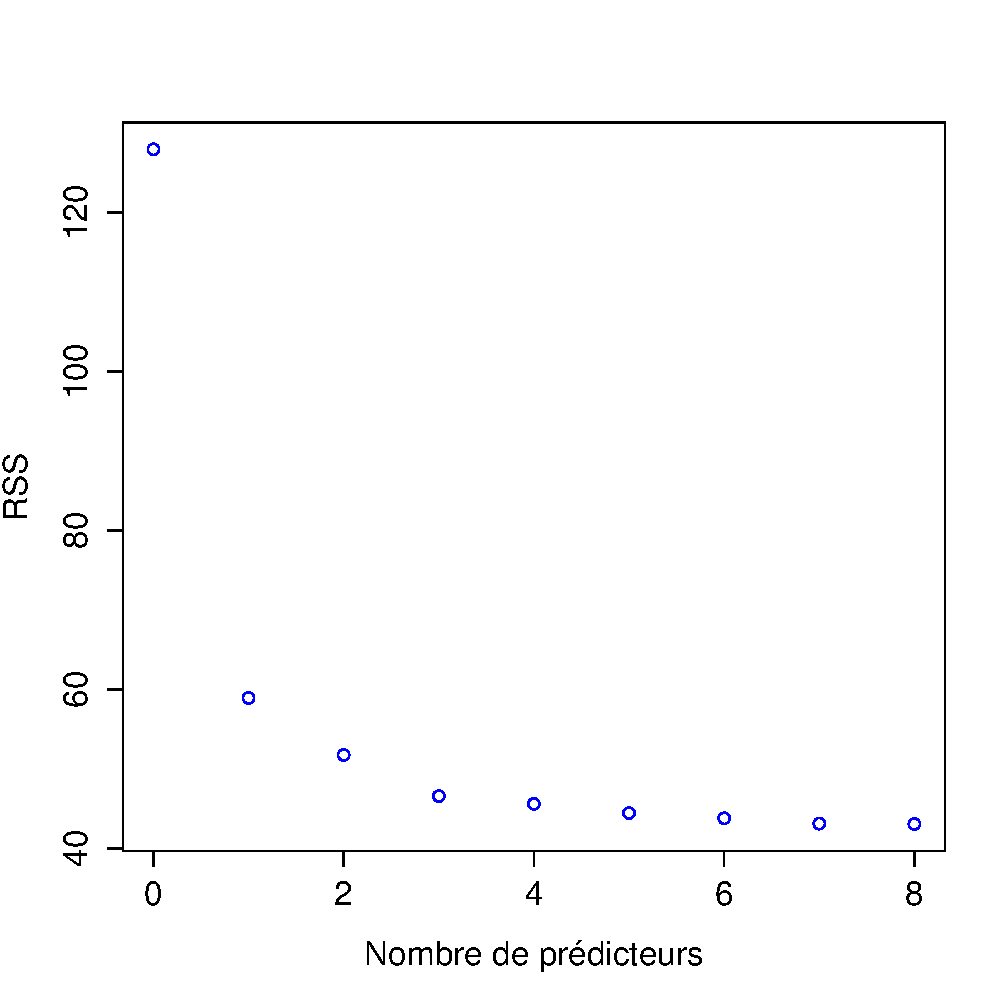
\includegraphics[scale=0.7]{rss.pdf}
\caption{Graphe des RSS en fonction du nombre de prédicteurs}
\end{center}
\end{figure}

On indique ci-dessous les sous-ensembles de prédicteurs qui réalisent le minimum de RSS, à nombre $k$ de prédicteurs fixé :
\begin{itemize}
\item $k = 0: \emptyset$
\item $k = 1: \{lcavol\}$
\item $k = 2: \{lcavol, lweight\}$
\item $k = 3: \{lcavol, lweigth, svi\}$
\item $k = 4: \{lcavol, lweight, lbph, svi\}$
\item $k = 5: \{lcavol, lweight, age, lbph, svi\}$
\item $k = 6: \{lcavol, lweight, age, lbph, svi, lcp\}$
\item $k = 7: \{lcavol, lweight, age, lbph, svi, lcp, pgg45\}$
\item $k = 8: \{lcavol, lweight, age, lbph, svi, lcp, gleason, pgg45\}$
\end{itemize}

\item Cette méthode ne permet pas de sélectionner le meilleur modèle, toutes tailles confondues, il ne permet que de déterminer le modèle qui "colle" le plus aux données, le nombre de prédicteurs étant fixé. Le meilleur modèle n'est pas nécessairement celui qui considère le plus de prédicteurs. En particulier, on n'évalue toujours pas la qualité des prédictions, qui est le seul critère qui importe véritablement. L'objectif de la split-validation est justement de tenir compte de ce critère pour affiner le choix du modèle.

\end{enumerate}


\section{Split-validation}

\begin{enumerate}

\item La split-validation consiste à séparer les échantillons en deux sous-ensembles :

\begin{itemize}
\item Une partie pour effectuer différentes régressions (ensemble d'apprentissage)
\item Une partie pour tester les différents modèles de régression possibles, et sélectionner celui qui produit les meilleures prédictions (ensemble de test)
L'ensemble de test permet donc de comparer les valeurs prédites aux valeurs mesurées.
\end{itemize}

\item 

\item Le meilleur modèle de taille 2 contient les prédicteurs $i = 1$ (lcavol) et $j = 2$ (lweight). lm(lpsa~.,data=pro[-valid,c(i,j,9)]) correspond au calcul de la régression sur l'ensemble d'apprentissage (-valid), en s'intéressant uniquement aux prédicteurs lcavol et lweight.

L'erreur d'apprentissage moyenne pour ce modèle est $0.503$. A noter que l'erreur est prise au sens des moindres carrés.

\item L'erreur de prédiction moyenne est $0.575$. On peut observer qu'elle est du même ordre de grandeur que l'erreur d'apprentissage moyenne.

\end{enumerate}



\end{document}

% TODO : parler du scrum master
